\documentclass[a4paper]{article} 

%% Language and font encodings
\usepackage[english]{babel}
\usepackage[utf8]{inputenc}
\usepackage[T1]{fontenc}
%% Sets page size and margins
\usepackage[a4paper,top=2cm,bottom=2cm,left=2.5cm,right=2.5cm,marginparwidth=1.75cm]{geometry}


%% Useful packages
\usepackage{amsmath}
\usepackage{graphicx}
\usepackage{tabularx}
\usepackage{xcolor}
\definecolor{tcdBlue}{RGB}{5, 105, 185}
\usepackage[colorlinks=true,allcolors=.,urlcolor=blue]{hyperref} % allowing hyperlinking of references. You can set the colour of the links or turn the colorlinks to false if no colour preferable. 
\usepackage[numbers]{natbib} % for Vancouver numbering style citation. Remove the [numbers] command for author-year Harvard style referencing. 


\usepackage{listings} % Add this package for code formatting
\usepackage{color}    % Add this package if you want to add color to your code

% Define colors for syntax highlighting
\usepackage{xcolor}
\definecolor{verylightgray}{rgb}{0.9,0.9,0.9}
\definecolor{commentcolor}{rgb}{0.5,0.5,0.5}
\definecolor{keywordcolor}{rgb}{0,0,1}
\definecolor{stringcolor}{rgb}{0.58,0,0.82}

% Configure the listings package
\lstset{ %
  language=Python,                     % the language of the code
  basicstyle=\ttfamily\small,          % the size of the fonts that are used for the code
  numbers=left,                        % where to put the line-numbers
  numberstyle=\small\color{lightgray},      % the style that is used for the line-numbers
  stepnumber=1,                        % the step between two line-numbers. If it's 1, each line will be numbered
  numbersep=5pt,                       % how far the line-numbers are from the code
  backgroundcolor=\color{verylightgray},       % choose the background color. You must add \usepackage{color}
  showspaces=false,                    % show spaces adding particular underscores
  showstringspaces=false,              % underline spaces within strings
  showtabs=false,                      % show tabs within strings adding particular underscores
  frame=single,                        % adds a frame around the code
  rulecolor=\color{black},             % if not set, the frame-color may be changed on line-breaks within not-black text
  tabsize=2,                           % sets default tabsize to 2 spaces
  captionpos=b,                        % sets the caption-position to bottom
  breaklines=true,                     % sets automatic line breaking
  breakatwhitespace=false,             % sets if automatic breaks should only happen at whitespace
  title=\lstname,                      % show the filename of files included with \lstinputlisting; also try caption instead of title
  keywordstyle=\color{keywordcolor},   % keyword style
  commentstyle=\color{commentcolor},   % comment style
  stringstyle=\color{stringcolor},     % string literal style
  escapeinside={\%*}{*)},              % if you want to add LaTeX within your code
  morekeywords={*,...}                 % if you want to add more keywords to the set
}


%% optional changes to the style. Comment (Ctrl+/) to remove these options. 
% change font to sans-serif fonts. 
\renewcommand{\familydefault}{\sfdefault}
% Format chapter headings appropriately to include tcd blue. 
\usepackage{titlesec}
\titleformat{\section}[hang]{\normalfont\Large\bfseries\color{tcdBlue}}{\thesection}{1em}{}{}


%% For nomenclature. Comment away if not used. 
% \usepackage{nomencl} % for nomenclature
% \usepackage{etoolbox} % to group nomenclature
% \usepackage{multicol} % for multiple columns in a page/table

\hyphenation{op-tical net-works semi-conduc-tor}

\begin{document}
\title{Exam report\\2024M12PY - Machine Learning with Python}
\author{Dries Luts, Bino Maiheu and Marijke Van De Steene\footnote{In alphabetic order}}
\date{2025-06-05}
\maketitle

\begin{abstract}
This document describes the exam project for the 2024M12PY UGain course on Machine Learning with Python taught by Bart Van Rompaye.
\end{abstract}


\section{Executive summary}

A brief executive summary

\section{Analysis report}

A detailed technical description of the data analysis, training and interpretation. 

\subsection{Data analysis and processing}

In figure \ref{fig:score_histograms} we see some interesting things appear. According to \citet{bishop2006pattern}, data preprocessing is a crucial step in machine learning.

\begin{figure}[!h]
    \centering
    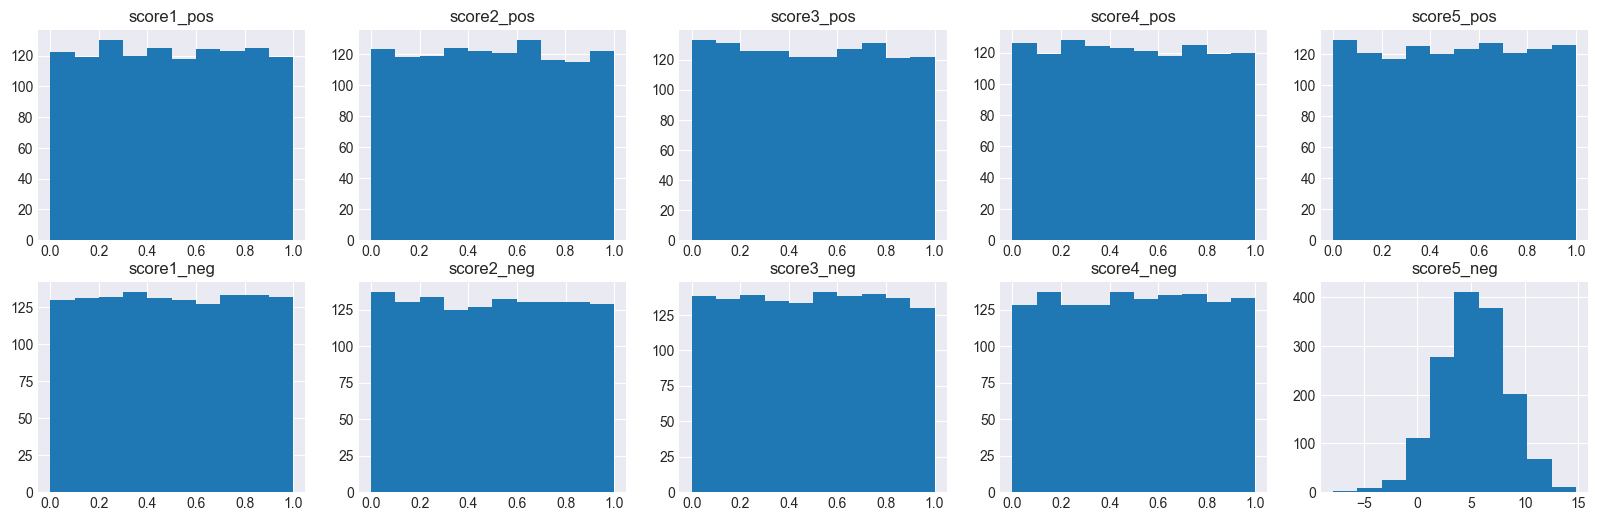
\includegraphics[width=1.0\textwidth]{figs/score_histograms.png}
    \caption{Histograms for the positivity and negativity scores by the 5 other hotels. We clearly see
    that the negativity scores for hotel 5 were not yet transformed to quantiles.}
    \label{fig:score_histograms}
\end{figure}

\subsection{Model training}


\begin{lstlisting}
def factorial(n):
    """
    Return the factorial of a number.
    
    Args:
        n (int): The number to calculate the factorial of.
    
    Returns:
        int: The factorial of the number.
    """
    if n == 0:
        return 1
    else:
        return n * factorial(n-1)

print(factorial(5))
\end{lstlisting}
\subsection{Results and discussion}



%% References
\bibliographystyle{unsrtnat} % Vancouver reference style (numbering). 
% \bibliographystyle{agsm} % Harvard reference style (author-year). 
\bibliography{bibliography}
\addcontentsline{toc}{section}{Bibliography}

\end{document}